\documentclass[../thesis.tex]{subfiles}
\begin{document}

\section{Cohn and Umans Matrix Multiplication}\label{sec:CandU}
Here, we present the Cohn and Umans \cite{CohnOld}\cite{CohnNew} framework for fast matrix multiplication. We begin by recalling the notion of a \textbf{finite group} $G$, and the \textbf{group algebra} $\CC[G].$ These structures are the backbone of Cohn and Umans' algorithm. The reader is referred to Dummit and Foote \cite{abs} for a background on modern algebra. 

\subsection{The Embedding of Matrices}
The first stage of the Cohn and Umans matrix multiplication algorithm is producing a representation for matrices. Suppose we have a matrix with entries in $\CC$,
\begin{equation*}
    A = \begin{bmatrix}1 & 2 \\ 3 & 4\end{bmatrix}.
\end{equation*}
We want to \textbf{embed} this matrix in the group algebra $\CC[G]$, where $G$ is a group containing at least four elements. Let $g_1,g_2,g_3,g_4\in G$ be distinct elements of the group $G$. We obtain the following representation:
\begin{equation}\label{eq:matrixembedding}
    \Bar{A} = 1g_1 + 2g_2 + 3g_3 + 4g_4\in\CC[G].
\end{equation}
The matrix $A$ is now expressed as the element $\Bar{A}$ of the group algebra $\CC[G]$, where $\CC$ is the base field of the matrix $A.$ We remark that this is a naive description of the embedding. For a working implementation of matrix multiplication our group and embedding strategy must satisfy the \textit{triple-product property}. For now, we highlight the features of this embedding structure that are necessary for the topic.

Elements of the group algebra $\CC[G]$ are formal sums much like a polynomial in an indeterminate $x.$ The coefficients in Equation \ref{eq:matrixembedding} are elements of the field $\CC$, defined with the usual multiplication and addition operations from $\CC$. The group elements are defined with a multiplication operation between them. However, field elements and group elements have no operations defined between them. 

Elements of a group algebra can be multiplied similarly to polynomials:
\begin{equation}\label{eq:groupalgebraproduct}
    \Bar{A}\Bar{B} = \Big(\sum_{i=1}^n \Bar{A}_ig_i\Big)\Big(\sum_{j=1}^n \Bar{B}_jg_j\Big) = \sum_{i=1}^n\sum_{j=1}^n (a_ib_j)(g_ig_j).
\end{equation}
We remark that the transformation from a matrix to an element of a group algebra is invertible. With an appropriate choice of group for 2 matrices, and a correct embedding, we can compute their product in the algebra. We then apply the inverse transformation to recover the product matrix from the product of algebra elements.

\subsection{The Wedderburn-Artin Theorem}
The second stage of the Cohn and Umans algorithm is where speedups are realized. We rely on an application of the Wedderburn-Artin Theorem \cite{hypercomplexArt}\cite{hypercomplexWedd}, and we present this result in the context of this application.

Let $G$ be a finite group and $\CC[G]$ the group algebra. By the Wedderburn-Artin Theorem there exists an invertible function $\Phi$ such that,
\begin{equation}\label{eq:complexWAthm}
    \Phi: \CC[G] \longrightarrow \CC^{d_1\times d_1}\times\cdots\times\CC^{d_c\times d_c}
\end{equation}
for $d_i\in\NN.$ The right-hand-side is a block diagonal matrix of $d_i\times d_i$ matrices with entries in $\CC$. We call this form a \textbf{Weddeburn decomposition} of the group algebra $\CC[G]$, and each $\CC^{d_i\times d_i}$ is a \textbf{Wedderburn component}.

We can compute products of group algebra elements in this Wedderburn decomposition space. Let $\Bar{A},\Bar{B}\in\CC[G].$ Then,
\begin{equation}\label{eq:WedderburnProducts}
\begin{split}
    \Phi(\Bar{A})\Phi(\Bar{B})
                    &= \begin{bmatrix}
                        A_1 &\hdots &0 \\
                        \vdots & \ddots & \vdots\\
                        0 & \hdots & A_c
                    \end{bmatrix}
                    \begin{bmatrix}
                        B_1 &\hdots &0 \\
                        \vdots & \ddots & \vdots\\
                        0 & \hdots & B_c
                    \end{bmatrix}\\
                &= 
                \begin{bmatrix}
                    A_1B_1 & \hdots & 0\\
                    \vdots & \ddots & \vdots\\
                    0 & \hdots & A_cB_c
                \end{bmatrix}\\
                &= \Phi(\Bar{A}\Bar{B}).
\end{split}
\end{equation}
Each $A_i,B_i\in\CC^{d_i\times d_i}$ is a $d_i\times d_i$ matrix in with complex entries. These are the Wedderburn components. Since $\Phi$ is invertible, we can apply its inverse to $\Phi(\Bar{A}\Bar{B})$ and obtain the product $\Bar{A}\Bar{B}\in\CC[G].$

\subsection{Matrix Multiplication}
We now present the full Cohn and Umans \cite{CohnOld}\cite{CohnNew} algorithm. Let $G$ be a finite group, satisfying the \textit{triple-product property}, and  let $A,B$ be complex-valued matrices. We present \Call{MatrixMultiplication}{$A,B,G$} in Algorithm \ref{alg:CandUMatMult}. We also illustrate these steps graphically in Figure \ref{fig:CandUmatmult}.

\begin{figure}[t]
    \centering
    
    \label{fig:CandUmatmult}
     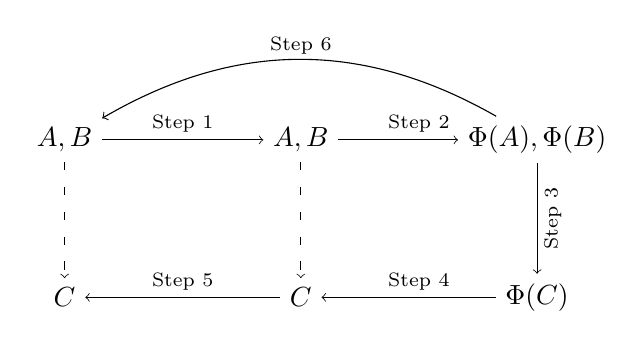
\begin{tikzpicture}[auto]
            \node(AB) at (0,2) {$A,B$};
            \node(ABbar) at (3,2) {$\Bar{A},\Bar{B}$};
            \node(ABphi) at (6,2) {$\Phi(\Bar{A}),\Phi(\Bar{B})$};
            \node(Cphi) at (6,0) {$\Phi(\Bar{C})$};
            \node(Cbar) at (3,0) {$\Bar{C}$};
            \node(C) at (0,0) {$C$};

            \node(phi) at (1.5,.2) {\scriptsize Step 5};
            \node(phiinv) at (4.5,.2) {\scriptsize Step 4};
            \node(phi) at (4.5,2.2) {\scriptsize Step 2};
            \node(embed) at (1.5,2.2) {\scriptsize Step 1};
            \node[rotate=90](waprod) at (6.2,1) {\scriptsize Step 3};
            \node(recur) at (3,3.2) {\scriptsize Step 6};
            
            \path[black, bend right][->] (ABphi) edge (AB);
            \draw[line width=.1mm, black][->] (AB) -- (ABbar);
            \draw[line width=.1mm, black][->] (ABbar) -- (ABphi);
            \draw[line width=.1mm, black][->] (ABphi) -- (Cphi);
            \draw[line width=.1mm, black][->] (Cphi) -- (Cbar);
            \draw[line width=.1mm, black][->] (Cbar) -- (C);
            \draw[line width=.1mm, black, loosely dashed][->] (AB) -- (C);
            \draw[line width=.1mm, black, loosely dashed][->] (ABbar) -- (Cbar);
        \end{tikzpicture}
        \caption{Cohn and Umans Matrix Multiplication}
\end{figure}

Speedups are realized during Step 3 and improved upon by Step 6. The former is the block diagonal matrix multiplication step. As shown in Equation \ref{eq:WedderburnProducts}, we can compute the matrix products of the block matrices pointwise. Each block has dimension $d_i\times d_i.$ We achieve improvements on the naive exponent $\omega = 3$ when the following inequality holds:
\begin{equation}
    \sum_{i=1}^k d_i^3 < n^3.
\end{equation}
Cohn and Umans have shown many group algebras afford a decomposition such that the inequality holds. However, we can improve on this inequality. Step 6 indicates a recursive call to the Cohn and Umans algorithm. Since computing the product of two block diagonal matrices is equivalent to computing individual products of the blocks, we further reduce the problem by decomposing the block sub-product. This leads to even more speedups. We show the recursive pattern in more detail on Line 11 of Algorithm \ref{alg:CandUMatMult}. Using this argument, Cohn and Umans were able to demonstrate a theoretical upper bound of $\omega = 2.41$ \cite{CohnNew}.  

Cohn and Umans give a rigorous treatment of Steps 1 and 5. Their computation is well-understood, and implementations have been produced by Anderson \cite{anderson}. Step 3 is also well-understood, the algorithm for which is naive matrix multiplication.

Steps 2 and 4 remain elusive. Algorithms for computing the Wedderburn-Artin theorem are computationally complex and niche. The package Wedderga \cite{wedderga} of the computational discrete algebra system GAP \cite{gap} is the closest we have found. However, the Wedderga implementation only returns the dimensions of the Wedderburn components. In an effort perform Cohn and Umans matrix multiplication, we implemented an algorithm which returns $\Phi$ as an explicit mapping of elements of a group algebra to matrices in the Wedderburn decompositions.

\begin{algorithm}[t]
\centering
\caption{Cohn and Umans Matrix Multiplication}\label{alg:CandUMatMult}
\begin{algorithmic}[1]
\Require $A,B\in\CC^{n\times n}$
\Require $\left|G\right| \ge n^2$
\Require $G$ is a group with the \textit{Triple-Product Property}
\Function{MatrixMultiplication}{$A,B,G$}
\If{\Call{dim}{$A$}$\leq 4$}\Comment{Base Case: No speedups in reduction}
    \State\Return $AB$
\EndIf
\State $\Bar{A}\gets$\Call{Embed}{$A,G$}\Comment{Embedding}
\State $\Bar{B}\gets$\Call{Embed}{$B,G$}
\State $\Phi\gets$\Call{ComputeWAThm}{G}\Comment{Define the Wedderburn-Artin Theorem mapping for $\CC[G]$}
\State $A_1,...,A_k\gets\Phi(\Bar{A})$\Comment{Compute the matrix blocks}
\State $B_1,...,B_k\gets\Phi(\Bar{B})$
\For{$i\in[1,k]$}
\State$C_i\gets$\Call{MatrixMultiplication}{$A_i,B_i,G'$} \Comment{Call with optimal group for dimensions}
\EndFor
\State $\Bar{C}\gets\Phi^{-1}(C_1,...,C_k)$\Comment{Inverse Wedderburn-Artin Theorem mapping}
\State $C\gets\Call{UnEmbed}{\Bar{C},G}$\Comment{Inverse embedding}
\State\Return $C$
\EndFunction
\end{algorithmic}
\end{algorithm}

\end{document}
